\documentclass[journal,12pt,twocolumn]{IEEEtran}

\usepackage{setspace}
\usepackage{gensymb}

\singlespacing


\usepackage[cmex10]{amsmath}
\usepackage{amsthm}

\usepackage{mathrsfs}
\usepackage{txfonts}
\usepackage{stfloats}
\usepackage{bm}
\usepackage{cite}
\usepackage{cases}
\usepackage{subfig}

\usepackage{longtable}
\usepackage{multirow}

\usepackage{enumitem}
\usepackage{mathtools}
\usepackage{steinmetz}
\usepackage{tikz}
\usepackage{circuitikz}
\usepackage{verbatim}
\usepackage{tfrupee}
\usepackage[breaklinks=true]{hyperref}
\usepackage{graphicx}
\usepackage{tkz-euclide}
\usepackage{float}

\usetikzlibrary{calc,math}
\usepackage{listings}
    \usepackage{color}                                            %%
    \usepackage{array}                                            %%
    \usepackage{longtable}                                        %%
    \usepackage{calc}                                             %%
    \usepackage{multirow}                                         %%
    \usepackage{hhline}                                           %%
    \usepackage{ifthen}                                           %%
    \usepackage{lscape}     
\usepackage{multicol}
\usepackage{chngcntr}

\DeclareMathOperator*{\Res}{Res}

\renewcommand\thesection{\arabic{section}}
\renewcommand\thesubsection{\thesection.\arabic{subsection}}
\renewcommand\thesubsubsection{\thesubsection.\arabic{subsubsection}}

\renewcommand\thesectiondis{\arabic{section}}
\renewcommand\thesubsectiondis{\thesectiondis.\arabic{subsection}}
\renewcommand\thesubsubsectiondis{\thesubsectiondis.\arabic{subsubsection}}


\hyphenation{op-tical net-works semi-conduc-tor}
\def\inputGnumericTable{}                                 %%
\lstset{
%language=C,
frame=single, 
breaklines=true,
columns=fullflexible
}
\begin{document}
\newtheorem{theorem}{Theorem}[section]
\newtheorem{problem}{Problem}
\newtheorem{proposition}{Proposition}[section]
\newtheorem{lemma}{Lemma}[section]
\newtheorem{corollary}[theorem]{Corollary}
\newtheorem{example}{Example}[section]
\newtheorem{definition}[problem]{Definition}

\newcommand{\BEQA}{\begin{eqnarray}}
\newcommand{\EEQA}{\end{eqnarray}}
\newcommand{\define}{\stackrel{\triangle}{=}}
\bibliographystyle{IEEEtran}
\providecommand{\mbf}{\mathbf}
\providecommand{\pr}[1]{\ensuremath{\Pr\left(#1\right)}}
\providecommand{\qfunc}[1]{\ensuremath{Q\left(#1\right)}}
\providecommand{\sbrak}[1]{\ensuremath{{}\left[#1\right]}}
\providecommand{\lsbrak}[1]{\ensuremath{{}\left[#1\right.}}
\providecommand{\rsbrak}[1]{\ensuremath{{}\left.#1\right]}}
\providecommand{\brak}[1]{\ensuremath{\left(#1\right)}}
\providecommand{\lbrak}[1]{\ensuremath{\left(#1\right.}}
\providecommand{\rbrak}[1]{\ensuremath{\left.#1\right)}}
\providecommand{\cbrak}[1]{\ensuremath{\left\{#1\right\}}}
\providecommand{\lcbrak}[1]{\ensuremath{\left\{#1\right.}}
\providecommand{\rcbrak}[1]{\ensuremath{\left.#1\right\}}}
\theoremstyle{remark}
\newtheorem{rem}{Remark}
\newcommand{\sgn}{\mathop{\mathrm{sgn}}}
\providecommand{\abs}[1]{\left\vert#1\right\vert}
\providecommand{\res}[1]{\Res\displaylimits_{#1}} 
\providecommand{\norm}[1]{\left\lVert#1\right\rVert}
%\providecommand{\norm}[1]{\lVert#1\rVert}
\providecommand{\mtx}[1]{\mathbf{#1}}
\providecommand{\mean}[1]{E\left[ #1 \right]}
\providecommand{\fourier}{\overset{\mathcal{F}}{ \rightleftharpoons}}
%\providecommand{\hilbert}{\overset{\mathcal{H}}{ \rightleftharpoons}}
\providecommand{\system}{\overset{\mathcal{H}}{ \longleftrightarrow}}
	%\newcommand{\solution}[2]{\textbf{Solution:}{#1}}
\newcommand{\solution}{\noindent \textbf{Solution: }}
\newcommand{\cosec}{\,\text{cosec}\,}
\providecommand{\dec}[2]{\ensuremath{\overset{#1}{\underset{#2}{\gtrless}}}}
\newcommand{\myvec}[1]{\ensuremath{\begin{pmatrix}#1\end{pmatrix}}}
\newcommand{\mydet}[1]{\ensuremath{\begin{vmatrix}#1\end{vmatrix}}}
\numberwithin{equation}{subsection}
\makeatletter
\@addtoreset{figure}{problem}
\makeatother
\let\StandardTheFigure\thefigure
\let\vec\mathbf
\renewcommand{\thefigure}{\theproblem}
\def\putbox#1#2#3{\makebox[0in][l]{\makebox[#1][l]{}\raisebox{\baselineskip}[0in][0in]{\raisebox{#2}[0in][0in]{#3}}}}
     \def\rightbox#1{\makebox[0in][r]{#1}}
     \def\centbox#1{\makebox[0in]{#1}}
     \def\topbox#1{\raisebox{-\baselineskip}[0in][0in]{#1}}
     \def\midbox#1{\raisebox{-0.5\baselineskip}[0in][0in]{#1}}
\vspace{3cm}
\title{ASSIGNMENT 5}
\author{SOWMYA BANDI}
\maketitle
\newpage
\bigskip
\renewcommand{\thefigure}{\theenumi}
\renewcommand{\thetable}{\theenumi}
Download all python codes from 
\begin{lstlisting}
\begin{lstlisting}
https://github.com/Sowmyabandi99/Assignment5/blob/main/Ass5/assignment5.py
\end{lstlisting}
%
Latex-tikz codes from 
%
\begin{lstlisting}
https://github.com/Sowmyabandi99/Assignment5/blob/main/Ass5/main.tex
\end{lstlisting}
%
\section{Question No 2.51}
Find the intervals in which the function 
\begin{align}
f(x) = x^2-4x+6 
\end{align}
%
is
%
\begin{enumerate}
\item increasing
\item decreasing
\end{enumerate}
%
\section{SOLUTION} 
Given equation can be written as
\begin{align}
y = x^2-4x+6      \label{eq1}
\\
\implies x^2-4x-y+6 =0
\end{align}
\begin{align}
\vec{x}^T\myvec{1 & 0 \\ 0 & 0}\vec{x}+ 2\myvec{2 \\ \frac{-1}{2}}\vec{x}+f&=0
\end{align}
Here,
\begin{align}
\vec{V}=\myvec{1 & 0 \\ 0 & 0},\vec{u}=\myvec{2 \\ \frac{-1}{2}},f=6  \label{eq2}
\end{align}
Using eigen decomposition on $\vec{V}$,
\begin{align}
\vec{V}&=\vec{P}\vec{D}\vec{P}^T
\\
where,\vec{D}&=\myvec{\lambda_1 & 0 \\ 0 & \lambda_2} = \myvec{0 & 0\\0 & 1}   \label{eq3}
\\
\vec{P}&=\myvec{\vec{p_1} & \vec{p_2}} =\myvec{0 & 1\\1 & 0}  \label{eq4}
\end{align}
The vertex of parabola $\vec{c}$ is given by
\begin{align}
\myvec{\vec{u}^T + \eta\vec{p_1}^T \\ \vec{V}}\vec{c} &= \myvec{-f \\ \eta\vec{p_1}-\vec{u}} \label{eq5}
\end{align}
\begin{align}
where,\eta=\vec{u}^T\vec{p_1}=\frac{-1}{2}  \label{eq6}
\end{align}
Substituting values from \eqref{eq2},\eqref{eq4} and \eqref{eq6} in \eqref{eq5}
\begin{align}
\myvec{-2 & -1 \\ 1 & 0 \\ 0 & 0}\vec{c} &= \myvec{-6 \\ 2 \\ 0} \label{eq7}
\end{align}
Removing last row and representing \eqref{eq7} as augmented matrix and then converting the matrix to echelon form,
\begin{align}
\myvec{-2 & -1 & -6\\1 & 0 & 2} 
\xleftrightarrow{R_1\leftarrow \frac{R_1}{-2}}\myvec{1 & \frac{1}{2} & 2\\1 & 0 & 2} 
\\
%\myvec{1 & \frac{1}{2} & 3 \\0 & \frac{-1}{2} & -1}
\xleftrightarrow{R_2\leftarrow R_2 -R_1}\myvec{1 & \frac{1}{2} & 3 \\0 & \frac{-1}{2} & -1}
\\
%\myvec{1 & \frac{1}{2} & 3 \\0 & 1 & 2}
\xleftrightarrow{R_2\leftarrow (-2R_2)}\myvec{1 & \frac{1}{2} & 3 \\0 & 1 & 2}
\\
%\myvec{1 & 0 & 2\\0 & 1 & 2}
\xleftrightarrow{R_1\leftarrow R_1 - \frac{R_2}{2}}\myvec{1 & 0 & 2\\0 & 1 & 2}   \label{eq8}
\end{align}
From $\eqref{eq8}$ it can be observed that,
\begin{align}
\vec{c} &= \myvec{2 \\ 2}
\end{align}
$\therefore$ From -$\infty$ to $\vec{c}$ the function is decreasing and from $\vec{c}$ to $\infty$ the function is increasing.
\begin{enumerate}
\item f is increasing in interval (2,$\infty$)
\item f is decreasing in interval (-$\infty$,2)
\end{enumerate}

Plot of Parabola-
\numberwithin{figure}{section}
\begin{figure}[ht]
    \centering
    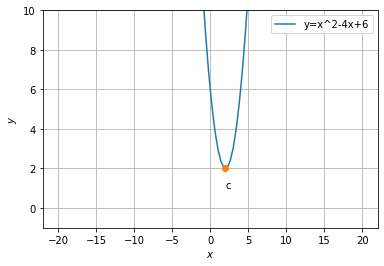
\includegraphics[width=\columnwidth]{Figure.png}
    \caption{Parabola}
    \label{fig:Prarabola}
\end{figure}    
\end{document}